\chapter{R\'esultats obtenus et limites de notre module de correction}

\section{R\'esultats: Un exemple illustrant les fonctionnalit\'es de notre module de correction}

Les exemples des chapitres pr\'ec\'edents \'etaient en fran\c{c}ais; l'exemple qui suit est en anglais afin de d\'emontrer le c\^ot\'e multilangue du module d'extension, et montrer aussi les fonctionnalit\'es de notre module.

L'interface de configuration d'une question de type \texttt{qtype\_essayhelper} est simple.
Si on prend seulement les configurations importantes, la configuration de base de la question, telle qu'illustr\'ee \`a la figure \ref{questionform_base}, est la m\^eme qu'avec les autres types de questions.

Rappel: le nom de la question est disponible pour l'enseignant seulement afin de retrouver la question dans la banque de questions Moodle, le texte de la question sera affich\'e \`a l'\'etudiant afin de r\'epondre \`a la question et la note par d\'efaut indique que la question est corrig\'ee sur 10 points.
\begin{figure}[htbp]
  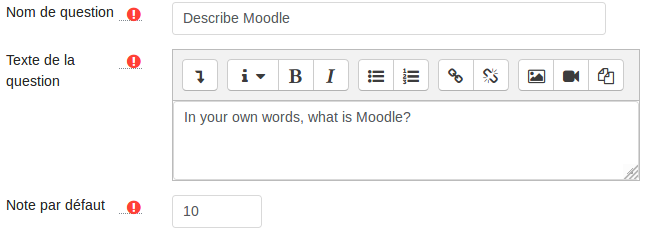
\includegraphics[scale=0.85]{images/questionform_base.png}
  \caption{Interface de configuration de base d'une question de type \texttt{qtype\_essayhelper}.}
  \label{questionform_base}
\end{figure}

La figure \ref{questionform_helper} montre les champs propres \`a \texttt{qtype\_essayhelper}.
On peut y voir les \'el\'ements suivants:
\begin{enumerate}
  \item La r\'eponse officielle de l'enseignant, qui sera affich\'ee \`a c\^ot\'e de la r\'eponse de l'\'etudiant. Le texte indiqu\'e dans cet exemple provient de la documentation Moodle\footnote{\url{https://docs.moodle.org/35/en/About_Moodle}};
  \item Les mots-cl\'es qui seront mis en \'evidence. Dans l'exemple donn\'e il y en a quatre: \textit{LMS}, \textit{open-source}, \textit{education} et \textit{personalisation};
  \item La langue pour la d\'etection des mots-cl\'es qui sera utilis\'ee par \texttt{phpstemmer}.
    Par d\'efaut la langue s\'electionn\'ee est la langue de l'utilisateur mais ici nous avons s\'electionn\'e manuellement l'anglais pour cet exemple.
\end{enumerate}
\begin{figure}[htbp]
  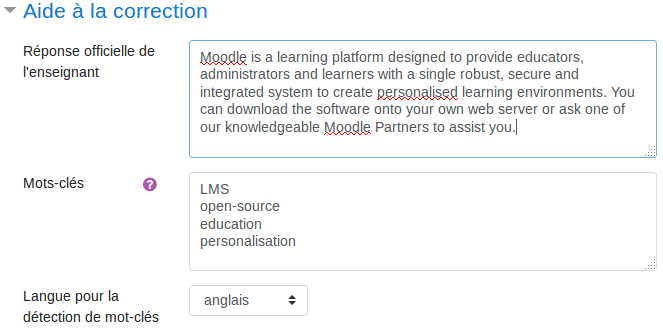
\includegraphics[scale=0.85]{images/questionform_helper.png}
  \caption{Interface de configuration pour l'aide \`a la correction d'une question de type \texttt{qtype\_essayhelper}.}
  \label{questionform_helper}
\end{figure}

Une fois que les \'etudiants r\'epondent, l'enseignant peut corriger avec l'aide \`a la correction en passant par le module d'extension de correction manuelle.
Un aperçu est disponible \`a la figure \ref{questionform_correction}.
Dans l'exemple, la r\'eponse de l'\'etudiant provient de Wikip\'edia\footnote{\url{https://en.wikipedia.org/wiki/Moodle}}.
On peut y voir les mots-cl\'es mis en \'evidence --- ils sont en caract\`eres gras et soulign\'es.
Pour le mot-cl\'e \textit{personalisation}, on peut voir le mot \textit{personalised} mis en \'evidence, car ils ont la m\^eme racine.
Pour le mot-cl\'e \textit{education}, on peut voir les mots \textit{educators} et \textit{education} mis en \'evidence, car ils ont tous la m\^eme racine \og educ \fg{} .

\begin{figure}[htbp]
  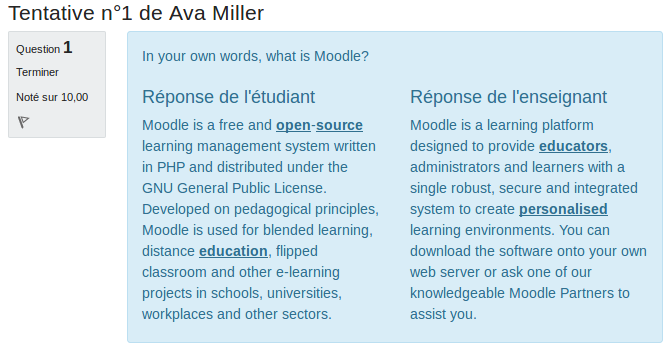
\includegraphics[scale=0.85]{images/questionform_correction.png}
  \caption{Interface de correction avec l'aide \`a la correction d'une question de type \texttt{qtype\_essayhelper}.}
  \label{questionform_correction}
\end{figure}

L'affichage de la r\'eponse de l'enseignant et de l'\'etudiant c\^ote \`a c\^ote, en plus des instructions au correcteur, devrait aider le correcteur dans sa t\^ache de correction.
De plus, la possibilit\'e de choisir la langue de racination permet aux enseignants d'utiliser l'aide \`a la correction dans la langue de leur choix.

\section{Limites et am\'eliorations possibles}
Malheureusement, aucun test n'a \'et\'e effectu\'e avec de vrai.e.s
\'etudiant.e.s dans un contexte r\'eel.  Bien que cela aurait \'et\'e
int\'eressant, plusieurs raisons expliquent pourquoi nous n'en avons
pas faits:
\begin{itemize}
  \item La professeure Fusaro, qui avait initi\'e l'id\'ee du projet avec mon directeur de recherche, le professeur Tremblay, est devenue Rectrice de l'UQAM durant le projet. Elle n'a donc pas pu collaborer \`a la mise en place d'un essai r\'eel;
  \item Les quelques cours que j'enseigne au C\'egep R\'egional de Lanaudi\`ere \`a Joliette n'ont pas d'examen ou d'atelier qui pourraient \^etre utilis\'es avec le module d'extension d'aide \`a la correction.
    Les examens sont de nature pratique (programmer une petite application, reproduire un document Microsoft Word, etc.) ce qui n'est pas utile dans ce contexte.
\end{itemize}

Un probl\`eme a \'et\'e d\'etect\'e vers la fin du projet: la s\'eparation du texte en mots peut poser probl\`eme.
Plus pr\'ecis\'ement, on s\'epare chaque mot en utilisant les symboles non alphanum\'eriques et les caract\`eres d'espacement.
Donc, le mot \og aujourd'hui \fg{} est consid\'er\'e comme deux mots, car l'apostrophe est un symbole non alphanum\'erique, alors que c'est en fait un seul mot.
Par contre, \og qu'autrui \fg{} est aussi consid\'er\'e comme deux mots, ce qui est correct dans ce cas.
De plus, comme le module d'extension supporte plusieurs langues, chaque langue comporte ses particularit\'es.
Par exemple, en anglais le mot \og \textit{wasn't} \fg{} est une compression des mots \og \textit{was} \fg{} et \og \textit{not} \fg{} ce qui ne sera pas bien g\'er\'e.
Toutefois, il nous semble que ce probl\`eme ne soit pas assez majeur pour cr\'eer des probl\`emes dans la majorit\'e des situations.
Ainsi, m\^eme si \og aujourd'hui \fg{} est consid\'er\'e comme deux mots, la mise en \'evidence se fera sur chacun de ces deux mots.
Et en anglais, les mots probl\'ematiques (comme \og \textit{wasn't} \fg{}) seront rarement utilis\'es comme mots-cl\'es.
Comme ce probl\`eme ne nous semble pas majeur et que la solution serait complexe \`a mettre en oeuvre --- par exemple, en rempla\c{c}ant la racination par la lemmatisation ou en faisant de l'analyse syntaxique ---, nous avons d\'ecidé de ne pas le traiter.

\`A la suite de l'analyse du probl\`eme pr\'ec\'edent, nous avons d\'ecouvert un deuxi\`eme probl\`eme.
Pour mettre en \'evidence les mots, on se base sur un dictionnaire qui associe le mot \`a la racine.
Si le mot-cl\'e est \og aimer \fg{} et le texte contient les mots \og aimera \fg{} et \og aimerait \fg{}, les deux mots seront mis en \'evidence.
Par contre, la partie du mot \og aimera \fg{} du mot \og aimerait \fg{} sera mise en \'evidence deux fois, car il contient l'autre mot qui doit \^etre mis en \'evidence.
La mise en \'evidence fait un simple remplacement de cha\^ine du mot par ce m\^eme mot entour\'e de balises \texttt{HTML} comme le d\'emontre l'exemple de code \ref{code:mots-cles}.
Une mise en \'evidence double ne sera pas diff\'erente visuellement d'une mise en \'evidence simple, car une balise de style \texttt{HTML} ou \texttt{CSS} dans une balise du m\^eme style ne fera pas de modification suppl\'ementaire.
En utilisant l'exemple pr\'ec\'edent, bien que \og aimerait \fg{} serait en partie mis en \'evidence deux fois, le mot ne sera soulign\'e qu'une seule fois.

Diverses am\'elioration pourraient aussi \^etre ajout\'ees au module d'extension.
Par exemple, la mise en \'evidence des mot-cl\'es est relativement simple; or, elle pourrait \^etre configurable via l'interface d'administration afin de changer le style de mise en \'evidence.
En ce moment la mise en \'evidence met simplement le mot en gras et soulign\'e.

La racination utilis\'ee est aussi limit\'ee~: le correcteur doit lire le contexte afin de confirmer si le mot-cl\'e est valide, probl\`eme qui pourrait \^etre \'elimin\'e avec un outil de lemmatisation.
De m\^eme, les mots-cl\'es originaux ne sont pas affich\'es au correcteur, ce qui pourrait \^etre un ajout int\'eressant.

Finalement, dans la planification initiale du projet, il \'etait pr\'evu de pouvoir comparer les textes des \'etudiants entre eux --- au lieu de seulement les comparer au texte de l'enseignant.
Dans un premier temps, nous voulions simplement afficher les r\'eponses des autres \'etudiants \`a la place de la r\'eponse de l'enseignant afin de comparer les r\'eponses semblables.
Par contre, cette id\'ee demandait une analyse syntaxique afin de trouver les r\'eponses semblables, ce qui sortait du cadre du projet.
Cet ajout pourrait \^etre un projet int\'eressant pour un futur \'etudiant.

Ces limitations font en sorte qu'il ne nous semble pas encore appropri\'e de soumettre
notre module au r\'epertoire officiel des modules d'extension Moodle.
Toutefois, apr\`es am\'eliorations, il pourrait devenir un ajout int\'eressant pour les enseignants et correcteurs du monde entier.

Signalons que
le code source de notre module est quand m\^eme disponible sur GitHub comme le stipule les r\`egles de d\'eveloppement Moodle, \`a l'adresse \url{https://github.com/Padreik/moodle-qtype_essayhelper}.
